% 0-Sphere Model series, Paper #63
% From Line Integral to Covariant Derivative: A Reader's Map of the Bridge
% from the 0-Sphere Model to Riemannian Curvature
% REVTeX 4-2 (APS/PRB). DOI: to be assigned on Zenodo deposit.
% ========================================
% Document Class and Package Setup
% ========================================
\documentclass[%
 reprint, amsmath,amssymb, aps, prb, ]{revtex4-2}
% Base packages
\usepackage{graphicx}
\usepackage{bm}
% Quantum-mechanics notation (physics package)
\usepackage{physics}
% Hyperlinks
\usepackage[colorlinks=true,
            linkcolor=blue, filecolor=blue, urlcolor=blue, citecolor=blue]{hyperref}
% Caption setup
\usepackage{caption}
\captionsetup[figure]{
    justification=raggedright, labelfont={bf}, name={Fig.}, labelsep=period }
\captionsetup[table]{
    labelfont={bf}, name={Table}, labelsep=period }
% Number equations per section
\numberwithin{equation}{section}
% Typography tuning
\tolerance=1000
\emergencystretch=1em
\hyphenpenalty=3000
\exhyphenpenalty=3000
\flushbottom
% Microtypography
\usepackage[final]{microtype}
\usepackage{ragged2e}  % for \justifying command
% booktabs rules: \midrule, \addlinespace, \bottomrule
\usepackage{booktabs}
\usepackage{enumitem}
% Theorem environment
\usepackage{amsthm}
\newtheorem{theorem}{Theorem}[section]
% --- paragraph heading: run-in italic with extra top skip for block readability ---
\makeatletter
\renewcommand\paragraph{%
  \@startsection{paragraph}{4}{\z@}%
    {3mm \@plus 1ex \@minus .2ex}%   before (block separator)
    {-1em}%                          after (negative keeps run-in)
    {\normalfont\normalsize\itshape}}
\makeatother
% Code listings with syntax highlighting
\usepackage{listings}
\usepackage{xcolor}
% Color definitions (light blue palette, academic)
\definecolor{backcolour}{rgb}{0.96,0.97,0.98}
\definecolor{deepblue}{rgb}{0,0,0.5}
\definecolor{deepgreen}{rgb}{0,0.5,0.3}
\definecolor{deepgray}{rgb}{0.4,0.4,0.4}
\definecolor{stringcolor}{rgb}{0.2,0.4,0.6}
% Python listing style
\lstdefinestyle{pythonstyle}{
    backgroundcolor=\color{backcolour}, commentstyle=\color{deepgreen}\itshape, keywordstyle=\color{deepblue}\bfseries, numberstyle=\tiny\color{deepgray}, stringstyle=\color{stringcolor}, basicstyle=\ttfamily\footnotesize, breakatwhitespace=false, breaklines=true, captionpos=b, keepspaces=true, numbers=left, numbersep=5pt, showspaces=false, showstringspaces=false, showtabs=false, tabsize=2, language=Python, frame=single, rulecolor=\color{deepgray} }
\lstset{style=pythonstyle}
% Internal phase notation
\newcommand{\iphase}{\theta}  % internal geometric phase = omega*t/2
\usepackage{tikz}
\usetikzlibrary{arrows.meta, calc, 3d, shadings, positioning, decorations.pathmorphing}
% --- Custom Macros ---
\newcommand{\omZB}{\omega_{\text{ZB}}}
\newcommand{\EphS}{E_{\text{ph}}}
\newcommand{\Egrad}{\Delta E_{\text{AB}}}
% Fundamental 1-form
% Field strength 2-form
\newcommand{\FF}{\mathbf{F}}
% Open Wilson line
\newcommand{\WL}{\mathcal{W}}
% Hodge dual
\newcommand{\hodge}{\star}

% ========================================
% Document Begin
% ========================================
\begin{document}

% ========================================
% Title, Author, and Date
% ========================================
\title{From Line Integral to Covariant Derivative: A Reader's Map of the Bridge from the 0-Sphere Model to Riemannian Curvature}

\author{Satoshi Hanamura}
\email{tensorphysik@gmail.com}

\date{June 20, 2026}

% ========================================
% Abstract
% ========================================
\begin{abstract}
This paper maps possible routes from the 0-Sphere model (0SM) to general relativity. In 0SM, interactions between two kernels are represented by a two-point action $\mathcal{S}(A,B)$ obtained along a thermal geodesic. The central question is whether spacetime geometry can emerge from this two-point structure. Two complementary routes are identified. The first treats $\mathcal{S}(A,B)$ as a Synge-like world function and explores the reconstruction of a spacetime metric $g_{\mu\nu}$. The second interprets the line-integral form $\mathcal{S}=\int_{\Gamma}A_{\mu}dx^{\mu}$ as a connection structure leading toward covariant derivatives, holonomy, and curvature. These routes correspond respectively to metric and connection approaches to emergent geometry. A key proposal is that curvature in 0SM may arise not from a congruence of spacetime geodesics, as in general relativity, but from a family of internal winding states associated with Thomas-type rotational dynamics. In this picture, the $\pi$-periodic spin-2 sector is identified as a candidate carrier of gravitational curvature. The paper does not claim a derivation of general relativity. Instead, it identifies the principal open problems required for such a derivation: the physical meaning of $A_{\mu}$, the tensorial status of the spin-2 winding sector, and whether the metric and connection routes converge to a common geometric structure. The result is therefore a research roadmap that clarifies the mathematical obstacles separating the current 0SM framework from a complete gravitational theory.
\end{abstract}

\maketitle

% ========================================
% Section 1: Introduction
% ========================================
\section{Introduction}
\label{sec:intro}

% ----------------------------------------
% Subsection 1.1: The picture in plain words
% ----------------------------------------
\subsection{The picture in plain words}

In the 0-Sphere model, matter is described by kernels and by the histories that connect one kernel to another. Over the previous drafts of this series, a clear sequence of ideas has settled into place. A kernel oscillates. That oscillation behaves like a source of heat, and heat spreads. Among all the ways the influence of kernel $A$ could reach kernel $B$, one path is singled out as the most efficient, and we call it the thermal geodesic. Finally, if we add up a certain quantity all along that path, we obtain a single number that depends only on the two endpoints $A$ and $B$. We call this number the two-point action and write it $\mathcal{S}(A,B)$. Because it is built by adding something up along a path, it is a line integral.

This paper sits at the current frontier of a long series, and a small number of its earlier results bear directly on what follows; we cite those, and only those, as they become relevant, reserving a fuller and citation-free account of the series' development for Sec.~\ref{sec:place}. Four threads matter here. The series introduced the thermal geodesic as the preferred exchange path between kernels, developing it as an extension of general relativity through internal thermodynamic structure~\cite{hanamura24,hanamura29}. It elevated the line integral of a connection one-form to the status of a fundamental observable in the line-integral trilogy~\cite{hanamura29,hanamura30,hanamura31}. It examined the derivative-order mismatch by which gauge theory and gravity assign physical meaning at different levels, identifying line integrals as their common observational layer~\cite{hanamura40,hanamura41}, and exhibited the gauge potential and the spacetime metric as twin outputs of a single open Wilson line~\cite{hanamura55}. And, most directly, it derived a helical trajectory whose fixed-endpoint line integral was identified with a generalized Synge world function, from which a spacetime metric emerges~\cite{hanamura51}. The present paper takes the next step in this arc: making explicit how that line integral connects to the covariant derivative and to curvature.

The goal that motivates the present paper is to connect this picture to general relativity, Einstein's theory of gravity~\cite{MTW1973}. General relativity is also a theory about distance and about paths, but it is built in what looks like the reverse order. It begins with a metric, which is the rule that tells you the distance between nearby points. From the metric it builds a connection, which is the rule for comparing directions at different places. From the connection it builds curvature, which measures how much the geometry bends. And from curvature it writes a field equation that ties the bending of space to the matter inside it.

So the 0-Sphere model and general relativity are walking toward each other from opposite ends. General relativity starts with the metric and works outward to a two-point notion of distance. The 0-Sphere model starts with a two-point quantity $\mathcal{S}(A,B)$ and must work back to a metric, and then onward to curvature. The question of this paper is simply: where, along that walk, is the hard part?

% ----------------------------------------
% Subsection 1.2: A short primer on the 0-Sphere Model, for the newcomer
% ----------------------------------------
\subsection{A short primer on the 0-Sphere Model, for the newcomer}
\label{subsec:primer}

The argument of this paper does not require the reader to have followed the series, only to hold a few ideas in mind. We collect them here in plain terms; nothing in this subsection assumes familiarity with any earlier draft, and the dictionary in Appendix~\ref{app:dictionary} gives a one-line gloss for every term used below.

\paragraph{The kernel.}
The basic object of the model is not a point particle but a \emph{kernel}: a small, structured source that oscillates. One can picture it as a tiny radiating body whose internal back-and-forth motion happens at a very high, fixed rhythm---the same rhythm that, elsewhere in the series, reproduces the electron's spin and its anomalous magnetic moment. For the purposes of this paper, only two facts about a kernel matter. It oscillates, and because it oscillates it radiates a heat-like influence into its surroundings.

\paragraph{The zero-sphere: two kernels, not one.}
The model is built not on a single kernel but on a \emph{pair} of them, labelled $A$ and $B$. This pair is the ``zero-sphere'' that gives the model its name: just as an ordinary sphere $S^2$ is the surface of a ball and a circle $S^1$ is its one-dimensional analogue, the zero-sphere $S^0$ is the lowest member of the family, and it consists of exactly two isolated points. Those two points are the two kernels. The crucial feature of two isolated points is that you cannot move continuously from one to the other while staying inside the set---there is a gap. Much of the model's structure comes from the physics that bridges that gap.

\paragraph{From oscillation to a preferred path.}
The two kernels are not silent. Each one's oscillation spreads outward as a heat-like disturbance, and the question the model keeps asking is: of all the ways the influence of kernel $A$ could reach kernel $B$, which one is actually taken? The answer is the most efficient route, the one that a heat-like, diffusive process naturally selects, and we call it the \emph{thermal geodesic}. It plays the same role here that a straight line plays on a flat sheet of paper, or that a great circle plays on the globe: it is the privileged path between two points, selected by the medium rather than imposed by hand.

\paragraph{The two-point action, and why it is a line integral.}
Once a unique preferred path from $A$ to $B$ exists, we can do something with it: we can add up a certain quantity all along it. The result is a single number that depends only on the two endpoints, and we call it the two-point action $\mathcal{S}(A,B)$. Because it is built by accumulating something step by step along a path, it is, by definition, a \emph{line integral}, which we write
\begin{equation}
\mathcal{S}(A,B) \;=\; \int_{\Gamma} A_\mu\,dx^\mu ,
\label{eq:S-primer}
\end{equation}
where $\Gamma$ is the thermal geodesic from $A$ to $B$ and $A_\mu$ is the quantity being accumulated. The reader should hold two questions lightly at this stage, because they become the spine of the whole paper: what kind of geometric object is the number $\mathcal{S}(A,B)$, and what kind of object is the integrand $A_\mu$? The first question leads to a metric; the second leads to a curvature; and the gap between asking them and answering them is exactly the territory this map charts.

\paragraph{The one habit of thought that unifies the series.}
If there is a single sentence that captures the model's stance, it is this: \emph{physically meaningful quantities live in accumulated histories along paths, not in local values at points}. A clock reading is the accumulation of proper time along a worldline; a quantum phase is the accumulation of a connection along a trajectory; an energy, in this model, is the history of a transport process rather than a number stored at a place. Holding this habit of thought makes the rest of the paper feel natural, because both of our two ``doors'' to curvature are, at heart, two different ways of asking what a path-accumulated quantity remembers about the geometry it passed through.

% ----------------------------------------
% Subsection 1.3: Where the hard part is, and is not
% ----------------------------------------
\subsection{Where the hard part is, and is not}

It is tempting to celebrate the line integral as the milestone. We will argue that this is the wrong place to plant the flag. A line integral, by itself, is one of the most common objects in physics. It is the work done by a force along a path, the circulation of a fluid, the flux threading a wire loop, the phase a quantum particle picks up. Arriving at ``a line integral'' tells us very little, because almost every theory has one.

What is special, and what genuinely smells like gravity, is the next move: to extract a \emph{metric} from a \emph{two-point} number like $\mathcal{S}(A,B)$. This exact move was made decades ago by J.~L.~Synge~\cite{Synge1960}, who showed that if you know the squared distance between every pair of nearby points, you can recover the metric by differentiating it twice, once with respect to each endpoint. The 0-Sphere drafts have repeatedly written a relation of just this shape. That is why we regard the metric as, in effect, already within reach.

If the metric is within reach, then the true obstacle is not the metric but the curvature. And here is the conceptual heart of the paper, stated in one sentence: \emph{curvature is never a property of a single path; it is a property of a whole family of neighboring paths}. A lone traveler walking a straight line learns nothing about whether the world is curved. Only when many travelers set out side by side, and we watch whether they drift together or apart, does curvature reveal itself. So the genuine wall for the 0-Sphere model is the step from one thermal geodesic to the entire bundle of nearby thermal geodesics. Cross that, and the distance to Synge, to bitensor calculus, and to Einstein's geometry shrinks dramatically.

% ----------------------------------------
% Subsection 1.4: What is genuinely new here, and what is re-presented
% ----------------------------------------
\subsection{What is genuinely new here, and what is re-presented}
\label{subsec:newold}

Because this is a map drawn across territory the series has already partly surveyed, honesty about provenance matters, and we state it plainly at the outset rather than leaving the reader to reconstruct it from citations. Two of the steps on this map are not new. The recovery of the metric from the two-point action by double differentiation---the first stage of the first door---was established in the earlier draft that introduced the helical trajectory and fixed-endpoint line integrals~\cite{hanamura51}. The reading of the line-integral integrand as a connection whose antisymmetric derivative is a curvature---the whole of the second door---was developed in the pair of drafts on the derivative-order mismatch between gauge theory and gravity~\cite{hanamura40,hanamura41}, building in turn on the line-integral trilogy~\cite{hanamura29,hanamura30,hanamura31}. We do not treat these as black boxes to be cited and abandoned. Because the 0-Sphere model is unfamiliar terrain, we judge it more useful to the reader to reproduce their essential content here, in self-contained appendices and in the reader's own hands, than to demand a detour through earlier papers; where we re-present a result, we say so explicitly and point to where it was first established.

What is genuinely new in this paper is fourfold, and we flag it so that the re-presented scaffolding is not mistaken for the contribution. First, we relocate the central difficulty and then correct the relocation: the line integral is behind us and the metric is essentially in hand, so the real wall is to find the \emph{family} in which curvature lives. Because the thermal geodesic between two kernels is unique~\cite{hanamura51}, that family cannot be a sheaf of neighbouring spatial paths---the standard geodesic congruence has no physical referent here---and we argue instead that it is the internal winding, the chirality degree of freedom~\cite{hanamura50}, realised as the Thomas-precession vortex on the internal $U(1)$ fibre bundle~\cite{hanamura48}. Second, we make this concrete by identifying the gravitational content of the curvature with the $\pi$-periodic, spin-2 component of that winding~\cite{hanamura48}, and by tracing how the same vortex drives the series' microscopic mechanism of gravity---fragment ejection and entropic synchronisation~\cite{hanamura49,hanamura34}---to a sharp prediction: that gravitational coupling \emph{freezes} rather than diverges at a horizon, because the Zitterbewegung clock that powers the vortex is redshifted to zero~\cite{hanamura22}. Third, we carry out a set of preliminary symbolic verifications of the roadmap steps (Appendix~\ref{app:checks}), one of which closes a flat-space consistency check that earlier work~\cite{hanamura51} had explicitly deferred. Fourth, we isolate the single decisive open problem on which both doors silently depend: the physical meaning of the connection one-form $A_\mu$. We note for honesty that an earlier version of this map mistakenly imported the van Vleck--Morette determinant and the Raychaudhuri equation as the load-bearing machinery for a spatial congruence; that machinery survives only as an optional mathematical cross-check (Appendix~\ref{app:congruence}), and the physical family is the internal one described above.

% ----------------------------------------
% Subsection 1.5: What this paper is, and how to read it
% ----------------------------------------
\subsection{What this paper is, and how to read it}

This paper is a map of the route, not a derivation of it. It is a perspective and program paper: its contribution is to locate the difficulty correctly and to lay out two concrete, complementary strategies for crossing it, together with checks that can be carried out next. We are careful throughout to mark which relations are imported by analogy from established geometry and which would have to be earned from 0-Sphere first principles.

We describe two doors into the same room. The first door, in Sec.~\ref{sec:distance} and Sec.~\ref{sec:bundle}, treats $\mathcal{S}(A,B)$ as a distance function, recovers the metric, and then watches a bundle of paths focus or spread to read off curvature. The second door, in Sec.~\ref{sec:connection}, reads the integrand of the line integral as a connection and obtains curvature from the failure of that connection to be path-independent. Section~\ref{sec:reconcile} explains why the two doors open into one geometry and states the open problem. Section~\ref{sec:einstein} describes what would still be needed to reach Einstein's equation, and Sec.~\ref{sec:outlook} gives a step-by-step roadmap.

To keep the main text readable, every piece of technical machinery is defined in a self-contained appendix, and each appendix is written so that it can be read on its own without recourse to earlier papers in the series. The reader can follow the whole argument for its ideas first, and consult Appendix~\ref{app:worldfn} for the distance-function and metric-recovery formulas, Appendix~\ref{app:congruence} for the bundle of paths and its focusing equations, and Appendix~\ref{app:connection} for connections, covariant derivatives, and curvature. Appendix~\ref{app:worked} works a single two-kernel example by hand, with explicit numbers, so that the most abstract claim of the second door can be checked on a sheet of paper; Appendix~\ref{app:checks} records the preliminary symbolic verifications; and Appendix~\ref{app:dictionary} is a short dictionary that translates, line by line, between the language of general relativity, the language of the 0-Sphere model, and ordinary words. Pointers to the appendices appear at each step. Where an appendix reproduces a result first established elsewhere in the series, it is labelled as such; the reproduction is deliberate, so that a reader new to the model need not assemble the picture from a stack of separate papers.

% ========================================
% Section 2: First door, part one: the two-point action as a distance function
% ========================================
\section{First door, part one: the two-point action as a distance function}
\label{sec:distance}

\paragraph{The everyday idea.}
Imagine you are handed a table that lists, for every pair of nearby towns, the squared straight-line distance between them. Remarkably, that table alone is enough to reconstruct the local map, including how distances stretch and shrink as you move around. The mathematical version of this statement is due to Synge: the squared geodesic distance between two points, viewed as a function of both points, is called the world function, and differentiating it once with respect to each endpoint and then bringing the points together returns the metric.

\paragraph{The 0-Sphere version.}
The 0-Sphere model hands us exactly such a two-point quantity, $\mathcal{S}(A,B)$, built by accumulating action along the thermal geodesic from $A$ to $B$~\cite{hanamura24,hanamura29,hanamura51}. The proposal of this series is to treat $\mathcal{S}(A,B)$ as playing the role of Synge's world function. If it does, the metric follows from the same double-differentiation,
\begin{equation}
g_{\mu\nu}(x) \;=\; \lim_{B\to A}\; \partial_{A\mu}\,\partial_{B\nu}\,\mathcal{S}(A,B).
\label{eq:metric-recon}
\end{equation}
The left-hand side is the metric at a point $x$; the right-hand side differentiates $\mathcal{S}$ once with respect to the first endpoint, once with respect to the second, and then lets the two endpoints merge at $x$. This identification of $\mathcal{S}(A,B)$ with a generalized world function, and the metric-recovery formula~\eqref{eq:metric-recon} that follows from it, were first set out in the earlier draft on the helical trajectory and fixed-endpoint line integrals~\cite{hanamura51}. We do not ask the reader to consult that draft: the precise meaning of every symbol, the analogy with Synge's $\sigma(x,x')$, the eikonal identity that underwrites the construction, and the reason the endpoint derivatives turn a scalar two-point number into a rank-two tensor, are all reproduced from first principles in Appendix~\ref{app:worldfn}, so that the first door can be understood here without leaving the page.

\paragraph{The order is reversed, and that is the whole point.}
It is worth pausing on the direction of the logic, because it is exactly opposite to the usual one. In standard general relativity the metric comes first: one is given $g_{\mu\nu}$, uses it to define what a geodesic is, and only then computes the geodesic distance between two points and packages it into Synge's world function. Metric $\to$ geodesic $\to$ two-point quantity. The 0-Sphere model runs this backward. It does not assume a metric. It begins from the physical claim that two points are joined by a thermal geodesic, given directly by kernel dynamics, and then asserts that a metric \emph{emerges} from that two-point structure through Eq.~\eqref{eq:metric-recon}. Two-point thermal geodesic $\to$ metric. In other words, in ordinary relativity the geometry is the input and the connecting path is the output, whereas in the 0-Sphere model the connecting path is the input and the geometry is the output. This inversion is precisely why the program is interesting and also why it cannot simply borrow Synge's results wholesale: it must earn the metric from the thermal geodesic, rather than presupposing one to define the geodesic.

\paragraph{Why this means the metric is ``in hand.''}
Relation~\eqref{eq:metric-recon} is not a fresh conjecture; it was already written down, and checked in the flat-space limit, in earlier work~\cite{hanamura51}, where it was shown that the symmetrized two-point action reduces in the absence of curvature to a quantity proportional to the proper time along the arc, so that its mixed endpoint derivatives return a matrix proportional to the Minkowski metric. That earlier draft also placed the construction in the context of the minimal-length ``bitensor'' programme of quantum gravity~\cite{Kothawala2023}, in which Synge's world function and the van Vleck--Morette determinant are precisely the two objects that carry the geometric information of a non-local two-point metric---a connection we will pick up and develop in the second half of the first door. For our purposes the point is that the metric is the leading, well-behaved content of the two-point action, and it is essentially solved. The work that remains is therefore not about the metric. It is about curvature, and curvature requires us to stop looking at a single path.

% ========================================
% Section 3: First door, part two: where the curvature actually lives
% ========================================
\section{First door, part two: where the curvature actually lives}
\label{sec:bundle}

\paragraph{A correction to the naive picture.}
In ordinary differential geometry one reads curvature off a \emph{family} of neighbouring geodesics: send many travellers side by side and watch whether they drift together. It is tempting to import that picture wholesale---to draw a bundle of nearby thermal paths between the two kernels and ask whether they focus---and an earlier draft of this map did exactly that. We now retract it, because it is physically false to the model. The thermal geodesic between kernels $A$ and $B$ is \emph{unique}: its existence and uniqueness were secured in earlier work~\cite{hanamura51} by the non-antipodality of the two kernels together with the Bonnet--Myers diameter bound, precisely so that the line integral $\mathcal{S}(A,B)$ is a genuine two-point functional. A unique path does not branch; there is no physical ensemble of side-by-side thermal geodesics to focus, and a literal picture of a bundle that ``starts apart and merges'' would contradict the very uniqueness the first door depends on. Borrowing the standard congruence here would be precisely the kind of import-by-analogy this paper has promised to avoid. Curvature is never a property of one object but of a family; the whole content of this section is that, in the 0-Sphere model, the family is a different one. Table~\ref{tab:replacement} states the replacement at a glance.

% ----------------------------------------
% Table 1
% ----------------------------------------
\begin{table}[h!]
\centering
\caption{\textbf{The replacement at the heart of the first door}}
\label{tab:replacement}
\renewcommand{\arraystretch}{1.35}
\begin{tabular}{p{3.7cm}p{3.9cm}}
\toprule
\textbf{General relativity} & \textbf{0-Sphere model} \\
\midrule
Geodesic congruence & Internal winding family \\
\addlinespace[0.15cm]
Geodesic deviation & Thomas-vortex deviation \\
\addlinespace[0.15cm]
Riemann curvature & Emergent winding curvature \\
\bottomrule
\end{tabular}
\end{table}

\paragraph{The family is internal, not spatial.}
The genuine family lives not in space but in the internal phase, and once that is seen the picture becomes both correct and concrete. The two kernels form a zero-sphere, and the internal oscillation that carries energy from $A$ to $B$ runs around a circle of phase $\theta\in[0,2\pi)$. Earlier work~\cite{hanamura48} showed that this single fact---$2\pi$-periodic internal motion---induces a principal $U(1)$ fibre bundle: the base is the phase circle $S^1$, the fibre at each $\theta$ is the internal complex phase, and the genuine degree of freedom is \emph{how the internal state winds} as it is carried along the one fixed thermal geodesic. The sign of that winding is the chirality $\chi=\mathrm{sign}(da/dt)$, a Lorentz-invariant topological binary classified by $\pi_1(S^1)=\mathbb{Z}$, which distinguishes electron from positron~\cite{hanamura50}; its magnitude is the internal excitation number. The ``family'' that reveals curvature is this fibre of windings over a single spatial path, not a sheaf of neighbouring paths in space (Fig.~\ref{fig:vortex}).

\paragraph{The winding is a real vortex.}
Crucially, the winding is not a bookkeeping abstraction; it is an energy circulation with substance. Because the thermal geodesic is an \emph{arc} in three dimensions, the photon sphere running along it is continuously accelerated transverse to its own motion, so its velocity $\mathbf v$ and acceleration $\mathbf a$ are never parallel and $\mathbf v\times\mathbf a\neq 0$. The result is a genuine internal angular velocity, the Thomas precession
\begin{equation}
\Omega_T(\theta)\;\propto\;\tfrac12\sin(2\theta),
\label{eq:omegaT}
\end{equation}
established in earlier work~\cite{hanamura19,hanamura49} and peaking at the midpoint $\theta=\pi/2$ of the $A\to B$ traversal. This $\Omega_T$ is the physical vortex: a real swirl of internal energy whose sense of rotation is the chirality. The connection that transports the phase around the fibre is the Berry connection of the $U(1)$ bundle, computed explicitly in~\cite{hanamura48} as $A_\theta(\theta)=\tfrac12\cos\theta$, whose holonomy around the internal circle is the coordinate-invariant Berry phase $\gamma_{\text{intrinsic}}=\pi$ that geometrically fixes $g=2$. The integrand of the first door's two-point action and the connection of the second door are, at bottom, this same object.

\paragraph{Where curvature appears, corrected.}
Curvature is therefore read not from the focusing of neighbouring spatial paths but from the winding structure of this internal bundle, and the hierarchy of internal periodicities makes the reading sharp. The same energy-conservation identity that produces the $2\pi$-periodic photon-sphere oscillation (the electromagnetic, spin-1 sector) produces a $\pi$-periodic component---the Thomas vortex $\Omega_T$---which earlier work~\cite{hanamura48} identifies, via the spin-periodicity relation $s=2\pi/T$, as the spin-2, and hence gravitational, candidate. The first door then reaches curvature by the clean inversion chain
\begin{align}
\underbrace{\mathcal{S}(A,B)}_{\text{two-point action}}
\;&\longrightarrow\;
\underbrace{g_{\mu\nu}=\partial_{A}\partial_{B}\mathcal{S}}_{\text{metric (Eq.~\ref{eq:metric-recon})}}
\notag\\[1.2ex]
&\longrightarrow\;
\underbrace{\Gamma^\rho{}_{\mu\nu}}_{\text{connection}}
\;\longrightarrow\;
\underbrace{R^\rho{}_{\sigma\mu\nu}}_{\text{curvature}},
\label{eq:inversion-first-door}
\end{align}
by ordinary differentiation of the emergent metric \emph{field}---which needs no physical congruence at all---while the specifically \emph{gravitational} content of that curvature is carried by the $\pi$-periodic winding sector of the internal bundle. We are careful to state this for what it is: at present it is a conceptual identification, not a derivation, and we name exactly the step that would promote it. \emph{The conceptual bridge from the internal winding to the Riemann tensor becomes a derivation only if the $\pi$-periodic Thomas sector is shown to transform as a rank-2 tensor under spacetime coordinate transformations}---the rank-2 tensor proof recorded as an explicit open task in the spin-2 and ejection drafts~\cite{hanamura48,hanamura49}. Until that is done, the winding is a candidate carrier of curvature, and we present it as such.

\paragraph{What this retires, and what it keeps.}
This retires the picture of a focusing spatial bundle, and with it the need to press the van Vleck--Morette determinant and the Raychaudhuri equation into service as physical machinery. Those remain available as a purely mathematical cross-check---once a metric field exists, the standard congruence calculus applies to it, and Appendix~\ref{app:congruence} records it in that spirit---but they are no longer the load-bearing step. What survives, and is sharpened, is the paper's central claim: a single object cannot reveal curvature. The correction is only about \emph{which} family does. It is not a sheaf of neighbouring paths in space; it is the fibre of internal windings---the chirality degree of freedom, realised physically as the Thomas vortex---over the one path that physically exists.

\begin{figure*}[t!]
\centering
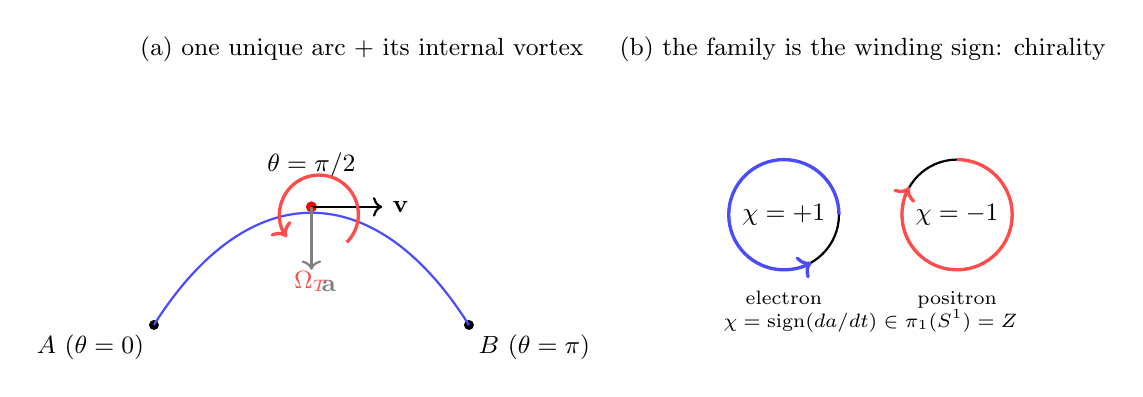
\begin{tikzpicture}[scale=1.0]
% --- panel (a): the A->B arc with the Thomas vortex ---
\node[anchor=west] at (-0.3,3.5) {\small (a) one unique arc + its internal vortex};
% chord A--B
\fill (0,0) circle (1.8pt); \node[below left] at (0,0) {\small $A$ ($\theta=0$)};
\fill (4,0) circle (1.8pt); \node[below right] at (4,0) {\small $B$ ($\theta=\pi$)};
% the arc
\draw[thick,blue!70] (0,0) .. controls (1.2,1.9) and (2.8,1.9) .. (4,0);
% photon sphere at midpoint
\fill[red] (2,1.5) circle (2pt);
\node[above] at (2,1.75) {\small $\theta=\pi/2$};
% velocity (tangent) and acceleration (transverse) at midpoint
\draw[->,thick,black] (2,1.5) -- (2.9,1.5) node[right] {\small $\mathbf v$};
\draw[->,thick,gray] (2,1.5) -- (2,0.7) node[below right] {\small $\mathbf a$};
% Thomas vortex curved arrow
\draw[->,very thick,red!70] (2.45,1.05) arc (-45:215:0.5);
\node[red!70] at (2.0,0.55) {\small $\Omega_T$};
% --- panel (b): chirality as winding sign ---
\begin{scope}[xshift=7.0cm]
\node at (2.0,3.5) {\small (b) the family is the winding sign: chirality};
% electron CCW
\draw[thick] (1.0,1.4) circle (0.7);
\draw[->,very thick,blue!70] (1.7,1.4) arc (0:300:0.7);
\node at (1.0,1.4) {\small $\chi=+1$};
\node[below] at (1.0,0.55) {\scriptsize electron};
% positron CW
\draw[thick] (3.2,1.4) circle (0.7);
\draw[->,very thick,red!70] (3.2,2.1) arc (90:-210:0.7);
\node at (3.2,1.4) {\small $\chi=-1$};
\node[below] at (3.2,0.55) {\scriptsize positron};
\node at (2.1,0.05) {\scriptsize $\chi=\mathrm{sign}(da/dt)\in\pi_1(S^1)=\mathbb{Z}$};
\end{scope}
\end{tikzpicture}
\caption{\textbf{The family that reveals curvature is the internal winding, not a sheaf of neighbouring spatial paths}}
\label{fig:vortex}
\vspace{0.4em}
\begin{minipage}{0.95\textwidth}
\justifying\small
(a) Between the two kernels there is exactly \emph{one} thermal geodesic---a unique arc, secured by non-antipodality and the Bonnet--Myers bound~\cite{hanamura51}; it does not branch. Because the arc is curved in three dimensions, the photon sphere running along it has velocity $\mathbf v$ and transverse acceleration $\mathbf a$ that are never parallel, so $\mathbf v\times\mathbf a\neq 0$ generates a real internal angular velocity, the Thomas precession $\Omega_T\propto\tfrac12\sin(2\theta)$, peaking at the midpoint $\theta=\pi/2$~\cite{hanamura19,hanamura49}. (b) The genuine degree of freedom is the \emph{sense} in which the internal phase winds---the Lorentz-invariant chirality $\chi=\mathrm{sign}(da/dt)$, classified by $\pi_1(S^1)=\mathbb{Z}$, distinguishing electron from positron~\cite{hanamura50}. Curvature lives in this winding structure of the internal $U(1)$ fibre~\cite{hanamura48}, not in any focusing of side-by-side paths; the $\pi$-periodic component of $\Omega_T$ is the spin-2 (gravitational) sector.
\end{minipage}
\end{figure*}

% ========================================
% Section 4: Second door: the line integral as a connection
% ========================================
\section{Second door: the line integral as a connection}
\label{sec:connection}

\paragraph{The everyday idea.}
Suppose you carry a compass needle across a landscape, always trying to keep it pointing ``the same way'' as you go. On flat ground, if you walk out and return by a different route, the needle comes back pointing where it started. On a curved surface it does not: carry it around a closed loop and it returns rotated. The rule for ``keeping it pointing the same way'' is called a connection, and the leftover rotation after a loop is, once again, curvature. The striking fact is that a connection is naturally described by exactly the kind of object the 0-Sphere model already has, namely something you integrate along a path.

\paragraph{The 0-Sphere version.}
The two-point action is written as $\mathcal{S}=\int_\Gamma A_\mu\,dx^\mu$, an integral of a quantity $A_\mu$ along the path $\Gamma$. In both electromagnetism and gauge theory, an object integrated along a path in this way is read as a connection~\cite{WuYang1975,AharonovBohm1959,Berry1984}: it tells a transported state how to adjust as it moves. The moment the model wrote $\mathcal{S}=\int A$, it had already stepped halfway into the language of connections. This reading is not introduced here for the first time. It is the content of the earlier pair of drafts on the derivative-order mismatch between gauge theory and gravity~\cite{hanamura40,hanamura41}, which argued that gauge theory and general relativity differ by exactly one derivative order in where they place physical meaning---gauge theory makes curvature the carrier of force, while general relativity makes the connection the carrier of force---and that line integrals of the connection are the common observational layer in which the two can be compared. Those drafts built, in turn, on the line-integral trilogy~\cite{hanamura29,hanamura30,hanamura31}, which first elevated the line integral $\Phi=\int_\Gamma\omega$ of a connection one-form to the status of the fundamental observable, and on the open-Wilson-line analysis that exhibited the gauge potential and the spacetime metric as twin outputs of the same path-ordered object~\cite{hanamura55}. So that the reader need not gather these threads from several papers, the connection, the path-ordered transport operator that carries a kernel state along $\Gamma$, the holonomy around a closed loop, and the covariant derivative whose failure to commute is curvature are all reproduced self-containedly in Appendix~\ref{app:connection}.

\paragraph{Where curvature appears here.}
If $A_\mu$ is a connection, its curvature is obtained by a simple antisymmetric derivative,
\begin{equation}
F_{\mu\nu} \;=\; \partial_\mu A_\nu - \partial_\nu A_\mu .
\label{eq:F-abelian}
\end{equation}
A nonzero $F_{\mu\nu}$ says something concrete and physical: the value of $\int_\Gamma A$ depends on \emph{which} path you take, not just on the endpoints. The line integral is path-dependent. For the 0-Sphere model this means the thermal exchange between $A$ and $B$ is route-sensitive, and accumulated route-sensitivity is the seed of curvature. When this is fed into the rule for comparing directions at neighboring points, the failure of that comparison to be order-independent is measured by the Riemann tensor (the full statement, including the commutator $[\nabla_\mu,\nabla_\nu]$, is in Appendix~\ref{app:connection}). Schematically, the second door is the chain
\begin{align}
\underbrace{\mathcal{S}=\int_\Gamma A_\mu dx^\mu}_{\text{line integral}}
&\;\longrightarrow\;
\underbrace{A_\mu}_{\text{connection}}
\notag\\
&\;\longrightarrow\;
\underbrace{F_{\mu\nu}}_{\text{path-dependence}}
\notag\\
&\;\longrightarrow\;
\underbrace{R^\rho{}_{\sigma\mu\nu}}_{\text{Riemann curvature}}.
\label{eq:gauge-chain}
\end{align}

\begin{figure*}[t!]
\centering
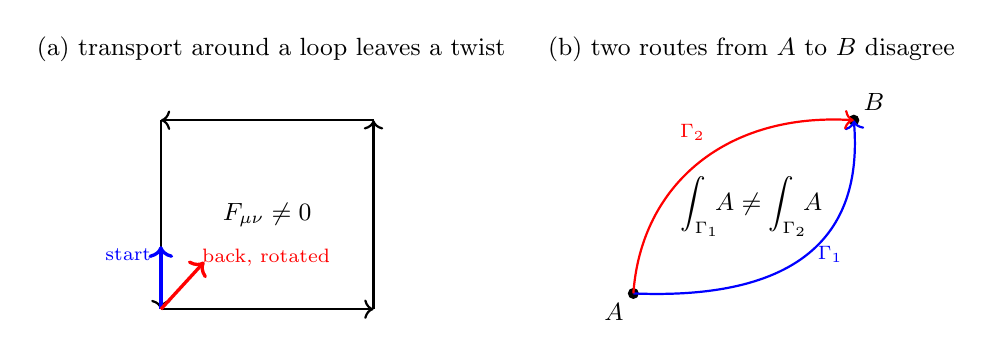
\begin{tikzpicture}[scale=1.0]
% --- panel (a): holonomy around a loop ---
\node at (1.6,3.5) {\small (a) transport around a loop leaves a twist};
\draw[thick,->] (0.2,0.2) -- (2.9,0.2);
\draw[thick,->] (2.9,0.2) -- (2.9,2.6);
\draw[thick,->] (2.9,2.6) -- (0.2,2.6);
\draw[thick,->] (0.2,2.6) -- (0.2,0.2);
% needle start (pointing up) and end (rotated)
\draw[blue,very thick,->] (0.2,0.2) -- ++(0,0.8);
\node[blue,left] at (0.2,0.9) {\scriptsize start};
\draw[red,very thick,->] (0.2,0.2) -- ++(0.55,0.6);
\node[red,right] at (0.6,0.85) {\scriptsize back, rotated};
\node at (1.55,1.4) {\small $F_{\mu\nu}\neq 0$};
% --- panel (b): two paths between A and B ---
\begin{scope}[xshift=6.0cm]
\node at (1.7,3.5) {\small (b) two routes from $A$ to $B$ disagree};
\fill (0.2,0.4) circle (2pt);
\node[below left] at (0.2,0.4) {\small $A$};
\fill (3.0,2.6) circle (2pt);
\node[above right] at (3.0,2.6) {\small $B$};
\draw[blue,thick,->] (0.2,0.4) .. controls (2.6,0.3) and (3.1,1.4) .. (3.0,2.6);
\node[blue] at (2.7,0.9) {\scriptsize $\Gamma_1$};
\draw[red,thick,->] (0.2,0.4) .. controls (0.3,1.8) and (1.4,2.7) .. (3.0,2.6);
\node[red] at (0.95,2.45) {\scriptsize $\Gamma_2$};
\node at (1.7,1.5) {\small $\displaystyle\int_{\Gamma_1}\!\!A \neq \int_{\Gamma_2}\!\!A$};
\end{scope}
\end{tikzpicture}
\caption{\textbf{Path-dependence of the line integral is the seed of curvature}}
\label{fig:holonomy}
\vspace{0.4em}
\begin{minipage}{0.95\textwidth}
\justifying\small
(a) Carrying a state around a closed loop while ``keeping it pointing the same way'' returns it rotated when the connection has nonzero curvature $F_{\mu\nu}$; the leftover twist is the holonomy. (b) Equivalently, the line integral $\int_\Gamma A_\mu dx^\mu$ from $A$ to $B$ gives different values along two different routes $\Gamma_1$ and $\Gamma_2$. The difference equals the flux of $F_{\mu\nu}$ through the region enclosed between the routes; a worked numerical example with explicit values is given in Appendix~\ref{app:worked}. For the 0-Sphere model, this is the statement that thermal exchange between two kernels is route-sensitive.
\end{minipage}
\end{figure*}

% ========================================
% Section 5: The two doors open into the same room
% ========================================
\section{The two doors open into the same room}
\label{sec:reconcile}

\paragraph{Not rivals, but two views.}
The first door starts from a two-point number and gets curvature from how a bundle of paths focuses. The second door starts from a path integral and gets curvature from how transport fails to close up. These are not competing theories. They are the two standard faces of one and the same Riemannian geometry: once you have a metric, it fixes a connection; once you have that connection, the leftover rotation it produces around a loop is the curvature whose contraction is exactly the focusing term from the first door. Table~\ref{tab:routes} lines up the familiar general-relativity backbone against its 0-Sphere reading along both faces, so a newcomer can see at a glance that the two columns end in the same place.

\paragraph{The same two doors, as two ways of moving the Wilson line.}
A structural analysis of the open Wilson line carried out elsewhere in the series~\cite{hanamura55} gives the two doors a sharper and more physical statement, and it is worth importing here because it says exactly what is being varied in each case. The line integral $\mathcal{S}=\int_\Gamma A_\mu\,dx^\mu$ has two endpoints and a path between them, and there are correspondingly two independent ways to perturb it. Holding the path fixed and displacing the two endpoints generates the first door: the response of $\mathcal{S}$ to endpoint displacement is what its mixed second derivative measures, and that derivative is the metric. Holding the endpoints fixed and deforming the path generates the second door: the response of $\mathcal{S}$ to a change of route is governed by $F_{\mu\nu}=\partial_\mu A_\nu-\partial_\nu A_\mu$, which is nonzero precisely when the integral is route-sensitive. Endpoint variation gives the metric; path variation gives the field strength. In Ref.~\cite{hanamura55} these are named the metric sector and the gauge (Maxwell) sector: two continuum descriptions grown from one and the same root, the Wilson line, by propagating its boundary data in two different directions---along endpoint pairs for the metric, along the path for the field strength. The gauge sector is not left as a slogan: a companion draft~\cite{hanamura54} carries the path-variation branch through in full, taking the field strength $F=d\Pi$ as a derived curvature of the integrand and recovering the four Maxwell equations, either as the identity $dF=0$ or as the stationarity of the action $S=-\tfrac{1}{4\mu_0}\!\int F\wedge\star F$, with classical electrodynamics emerging as the low-energy description valid once the observation scale exceeds the kernel separation. That framing is more cautious than the ``one room'' language of this section, because it presents the two doors as two sectors, gravitational and electromagnetic, rather than asserting outright that they terminate in a single curvature tensor. Whether they do ultimately collapse into one geometry---so that the gauge curvature $F_{\mu\nu}$ and the Riemann curvature $R^\rho{}_{\sigma\mu\nu}$ are two faces of one object---or whether they remain distinct sectors related only by a consistency condition, is precisely the unification question; the structural conditions under which such a collapse could occur are taken up separately in the series~\cite{hanamura60}. The present paper does not settle this. It insists only that the two doors are the two natural variations of a single object, which is why they are complementary rather than rival, and it locates the unresolved content honestly in the next paragraph.

\paragraph{The one genuinely open question.}
Putting the two doors together does not dissolve the difficulty; it sharpens it into a single question. Both doors quietly assume an interpretation of the integrand $A_\mu$. If $A_\mu$ is nothing more than a bookkeeping measure of how much heat flowed, then the connection door collapses and only the distance-function door survives. But if $A_\mu$ is a true connection, a thermal-flux potential that carries kernel state from $A$ to $B$, then $F_{\mu\nu}$ is the genuine path-dependence of thermal exchange, its accumulation forces transport to fail to close, and the bridge from $A_\mu$ to curvature becomes concrete and computable. So the operative question of this paper, stated plainly, is this: \emph{what is $A_\mu$, physically?} That, and not the line integral and not the metric, is the wall. Three earlier results narrow the question without answering it. A structural analysis of the open Wilson line~\cite{hanamura55} identifies the integrand as the Berry connection one-form of the 0-Sphere internal state bundle---the phase history carried by the photon sphere along its helical arc---and shows that its gauge freedom localizes entirely to the two kernel endpoints rather than spreading through space. That bundle is not merely named but constructed: the $2\pi$-periodic internal motion defines a principal $U(1)$ fibre bundle over the phase circle, on which the Berry connection is computed explicitly as $A_\theta(\theta)=\tfrac12\cos\theta$, with a coordinate-invariant holonomy $\gamma_{\text{intrinsic}}=\pi$~\cite{hanamura48}; this is the same one-form whose endpoint variation gave the metric and whose path variation gives the field strength. A study of phase accumulation along a single thermal geodesic~\cite{hanamura29} gives that same connection a concrete kinematic origin: along the real-space path between the two kernels, the non-commuting succession of Lorentz boosts generates a Thomas-precession connection $\Omega_T\propto \mathbf{a}\times\mathbf{v}$ whose line integral---not the curvature of the path, and not any surface integral---is the physically meaningful quantity. Between them, these results tell us a great deal about what $A_\mu$ \emph{does}: it is a connection one-form, induced by relativistic kinematics, that carries internal phase along an open worldline and whose redundancy lives at the endpoints. What they leave open is what it is \emph{made of}---the microphysical content of the thermal-flux potential, and in particular whether its symmetric, metric-generating part and its antisymmetric, spin-carrying part~\cite{hanamura51} share one origin. Stated more precisely, then, the wall is not whether $A_\mu$ is a connection---the series treats it as one---but what physical substance that connection encodes. Three readings remain on the table: $A_\mu$ as a \emph{thermal-flux potential}, as an \emph{information current}, or as a pure \emph{phase connection}; the decisive task is to settle among them. We stress the payoff of doing so, because it bounds the problem. \emph{Once $A_\mu$ is identified, the subsequent steps belong largely to standard differential geometry.} The difficulty is therefore not unbounded; it is concentrated at this single point. In the present state of the model $A_\mu$ is, if anything, less defined than the Riemann tensor that sits downstream of it, and that inversion---the foundation being less settled than the structure built on it---is exactly why we name $A_\mu$, and not the curvature, as the bottleneck.

\paragraph{A check we can do before answering it.}
There is a useful consistency test that does not require settling the interpretation first. The metric recovered in Sec.~\ref{sec:distance} determines its own natural connection (the Levi-Civita connection). The integrand $A_\mu$ determines a connection directly. The two doors are mutually consistent only if these two connections agree, up to the harmless relabeling freedom called gauge. Checking whether they agree, or characterizing any controlled disagreement as ``torsion,'' is a concrete next task that can be done without first resolving the full meaning of $A_\mu$.


% ----------------------------------------
% Table 2
% ----------------------------------------
\begin{table*}[t!]
\centering
\caption{\textbf{Two doors to the same curvature, told side by side}}
\label{tab:routes}
\renewcommand{\arraystretch}{1.4}
\begin{tabular}{p{3.5cm}p{5.5cm}p{6.5cm}}
\toprule
\textbf{Stage} & \textbf{First door (distance function)} & \textbf{Second door (connection)} \\
\midrule
What you start with
& The two-point action $\mathcal{S}(A,B)$, read as a squared-distance function
& The line integral $\mathcal{S}=\int_\Gamma A_\mu dx^\mu$, read as transport \\
\addlinespace[0.3cm]
First geometric object
& The metric $g_{\mu\nu}=\partial_{A\mu}\partial_{B\nu}\mathcal{S}$
& The connection $A_\mu$ \\
\addlinespace[0.3cm]
The clue to curvature
& Whether a bundle of paths stays even (the determinant $\Delta$)
& Whether the integral is path-independent (the field strength $F_{\mu\nu}$) \\
\addlinespace[0.3cm]
How curvature is read off
& Focusing of neighboring paths (Raychaudhuri)
& Failure of transport to close (the commutator $[\nabla_\mu,\nabla_\nu]$) \\
\addlinespace[0.3cm]
Curvature obtained
& Ricci tensor $R_{\mu\nu}u^\mu u^\nu$
& Riemann tensor $R^\rho{}_{\sigma\mu\nu}$ \\
\addlinespace[0.2cm]
\bottomrule
\end{tabular}
\vspace{0.2cm}
\begin{minipage}{0.95\textwidth}
\justifying\footnotesize
Both columns are intended to end in the same Riemannian curvature: the Ricci tensor in the left column would be the relevant contraction of the Riemann tensor in the right column. The two doors are complementary descriptions of one geometry. The program needs both, because the distance-function door connects most naturally to the matter content (through the stress-energy that sources gravity), while the connection door gives the most direct physical reading of the line integral the model already possesses. Whether the two columns truly terminate in a single curvature, or in two sectors sharing one root, is itself an open question, sharpened immediately below and grounded in the structural analysis of Ref.~\cite{hanamura55}.
\end{minipage}
\end{table*}


\paragraph{The decisive open problem.}
We end this section by stating, as plainly as we can, the question on which the whole programme turns---not because we can answer it, but because naming it precisely is the main service this map can render. \emph{Do the metric sector and the connection sector converge to the same curvature structure?} The first door, by endpoint variation, builds a metric and hence a curvature $R^\rho{}_{\sigma\mu\nu}$ from $\partial_A\partial_B\mathcal{S}$; the second door, by path variation, builds a field strength $F_{\mu\nu}$ from the same integrand. The structural analysis of the open Wilson line presents these as two distinct continuum sectors---gravitational and electromagnetic---grown from one root~\cite{hanamura55}, and does not, by itself, guarantee that they terminate in a single geometry. The convergence has a precise criterion: the Levi-Civita connection determined by the recovered metric must coincide, up to gauge, with the connection determined directly by $A_\mu$; any irreducible discrepancy is torsion. Whether that criterion is met---whether the two doors open into one room or into two adjacent rooms joined by a torsion corridor---is, in our view, the central unresolved question of the 0-Sphere approach to gravity. It is not a weakness of the framework but its focus, and everything downstream of it is contingent on its answer.

% ========================================
% Section 6: From the vortex to a force, and a prediction at the horizon
% ========================================
\section{From the vortex to a force, and a prediction at the horizon}
\label{sec:vortex-force}

The internal vortex of Sec.~\ref{sec:bundle} is not only the place where curvature is read; in the series it is also the engine of the gravitational interaction itself, and following that thread to its end yields a prediction that distinguishes the model sharply from general relativity. We trace it here because it gives the reader a physical picture of what the abstract ``gravitational sector'' actually does, and because it shows that the winding degree of freedom is doing real work.

\paragraph{From curvature to a force.}
The chain is short and entirely made of pieces the series has already built. The arc-curvature of the unique $A\to B$ geodesic makes $\mathbf v\times\mathbf a\neq 0$ and so generates the Thomas vortex $\Omega_T\propto\tfrac12\sin(2\theta)$, whose outward stress peaks at the midpoint $\theta=\pi/2$. For an internally excited kernel this stress saturates the geometric binding floor $E_0/2$ and ejects a photon-sphere fragment carrying one quantum $\hbar\omega$~\cite{hanamura49}. The fragment is absorbed by a neighbouring kernel, nudging the two toward entropic phase synchronisation; the synchronisation energy $\Delta E_{\text{sync}}=\hbar(\nu_b-\nu_a)$ converts into a translational drift, an effective free-fall acceleration $g_{\text{eff}}=\tfrac{1}{\Delta t}\sqrt{2\Delta E_{\text{sync}}/m}$~\cite{hanamura34}. Gravity, in this reading, is the macroscopic residue of neighbours exchanging the ejected fragments of each other's vortices. Two features matter for the present map. First, the smaller the arc radius---the tighter the vortex, the larger its curvature---the stronger the Thomas stress and the more readily a fragment is ejected, so the winding geometry directly modulates the coupling. Second, the coupling is weak not because the force is intrinsically feeble but because ejection is \emph{rare}: its probability per cycle is suppressed by a factor $\epsilon_2\epsilon_3\sim10^{-5}$, which is the series' account of why gravity is so many orders of magnitude weaker than electromagnetism~\cite{hanamura34,hanamura49}.

\paragraph{A prediction: the coupling freezes, rather than diverges, at the horizon.}
Now push the same chain into a strong gravitational field. The Zitterbewegung that drives the whole mechanism is an internal clock, and an internal clock redshifts: in a Schwarzschild field the proper-time rate is $d\tau/dt=\sqrt{1-2GM/rc^2}$, so as one approaches the horizon $r\to 2GM/c^2$ the internal frequency, and with it the transverse speed $v_{\text{ZB}}$, is driven to zero~\cite{hanamura22}. But the vortex strength scales as $\Omega_T\propto v_{\text{ZB}}^2$, so as $v_{\text{ZB}}\to 0$ the vortex stress vanishes and ejection ceases: the TPE-to-kinetic conversion that the whole mechanism depends on shuts down. The model therefore predicts that gravitational \emph{coupling}, read as the rate of fragment exchange, does not diverge at the horizon as the curvature of general relativity does---it \emph{freezes out}. Combined with the curvature-tightening of the previous paragraph, the force is non-monotonic in field strength: it strengthens as the vortex tightens, then collapses as the redshift freezes the internal clock, leaving a particle that is internally static and causally decoupled at the horizon---the ``hard stone'' limit in which a vanishing internal flexibility leaves matter deaf to the surrounding geometry~\cite{hanamura53}. This is a structural prediction, not a quantitative one, and we flag it as such; but it is a clean, in-principle-testable point of divergence from general relativity, and it follows from machinery the series already possesses.

\paragraph{Honesty about status.}
None of this is claimed as derived. The quantitative law connecting the arc curvature to the Thomas stress, and that stress to an ejection rate, is an explicit open task in the ejection paper~\cite{hanamura49}; whether the emergent metric of the first door is the same geometry that the ejected-fragment statistics build is the most ambitious open question of that programme. We include the chain because it shows that the winding degree of freedom which replaced the discarded spatial bundle is not an ornament: it is, in the series' own architecture, the carrier of the gravitational interaction, and it makes a prediction.

% ========================================
% Section 7: What it would take to reach Einstein's equation
% ========================================
\section{What it would take to reach Einstein's equation}
\label{sec:einstein}

Once the Ricci tensor is available from either door, the remaining objects of general relativity are essentially algebraic, and we summarize them so the destination is explicit. Tracing the Ricci tensor with the metric gives the Ricci scalar $R$, and combining the two gives the Einstein tensor
\begin{equation}
G_{\mu\nu} \;=\; R_{\mu\nu} - \tfrac12\,R\,g_{\mu\nu},
\label{eq:einstein-tensor}
\end{equation}
which has the special property of being automatically conserved. The destination of the whole program is the Einstein field equation
\begin{equation}
G_{\mu\nu} \;=\; 8\pi\,T_{\mu\nu},
\label{eq:efe}
\end{equation}
where $T_{\mu\nu}$ is the stress-energy, the content that tells gravity how strongly to bend.

It is worth being honest about what \eqref{eq:efe} still demands, since this paper does not supply it. Two things are required. First, geometrically, the curvature produced by either door must assemble into the specific conserved combination on the left of \eqref{eq:einstein-tensor}; the model does not yet guarantee this, and it must be shown rather than assumed. Second, physically, there must be a stress-energy $T_{\mu\nu}$ built from kernel content whose conservation matches the geometric side. The two-point action is the natural source of both, since the same $\mathcal{S}(A,B)$ that yields the metric should, through its higher-order behavior near coincidence, also supply the energy content on the right-hand side. Closing this loop is what it would mean for the 0-Sphere model to truly reach general relativity, and it is left to later drafts.

There is a subtlety here that the series has already anticipated, and naming it sharpens what ``reaching Einstein's equation'' would and would not mean. The capstone of the line-integral trilogy~\cite{hanamura31} already proposed the hierarchy that frames this: connection and proper time are the central variables, line integrals of the connection along thermal geodesics are the primary observables, the Einstein field equation enters as a consistency check derived from those accumulated connections, and curvature is a secondary descriptor of loop-level noncommutativity. A subsequent draft~\cite{hanamura30} developed this into a sharper claim: in a framework where physical observables are accumulated histories along worldlines, the Einstein field equation is most naturally read not as a generative law in which matter dictates geometry, but as an \emph{a posteriori} consistency condition---a global checksum---verifying that the independently accumulated phase histories of many worldlines fit together into a single coherent geometry. That draft makes the inversion precise. The primary geometric statement is taken to be the contracted Bianchi identity $\nabla^\mu G_{\mu\nu}\equiv 0$, which holds as a pure identity of the geometry; the conservation law $\nabla^\mu T_{\mu\nu}=0$ then follows as a \emph{consequence}, the requirement that the effective stress-energy read off from accumulated phase be compatible with that geometry, rather than as an independently imposed law. In this reading the stress-energy tensor is demoted from a causal agent to a descriptive quantity: each worldline $\gamma_i$ contributes its own phase history $\Phi_i=\int_{\gamma_i}\omega_i$ independently and locally, and the Einstein equation does not act on any single contribution but verifies that their aggregate is globally coherent. On that reading, the demand that the curvature assemble into the conserved Einstein tensor is not an extra dynamical postulate bolted onto the model; it is the statement that the family of thermal geodesics is mutually consistent, which is exactly the congruence-level question raised by the first door. The two halves of this paper and the checksum reading therefore point at the same object from two sides: the Raychaudhuri focusing of the congruence is the local face of the same global self-coherence that the Einstein equation, read as a checksum over the family of phase histories $\{\Phi_i\}$, enforces in the large. Likewise, the existence of a lower bound on the kernel separation, which keeps the two-point action from degenerating to a trivial zero-length argument, is supplied within the series by the geometric energy floor of the half-quantum result~\cite{hanamura46} together with the Bonnet--Myers diameter bound on the photon-sphere domain~\cite{hanamura51}, rather than being inserted by hand. We record these connections not because they close the loop---they do not---but because they show that the missing pieces of \eqref{eq:efe} are not arbitrary: each one has a natural home in structures the model has already built.

% ========================================
% Section 8: Outlook and roadmap
% ========================================
\section{Outlook and roadmap}
\label{sec:outlook}

We regard this paper as having relocated the problem rather than solved it, and we think the relocation is itself worth recording. The line integral is behind us. The metric is essentially in hand through Eq.~\eqref{eq:metric-recon}. The wall is the passage from a single thermal path to the geometry of the whole bundle of paths, which is the same wall as the question of what the connection $A_\mu$ physically means. The next steps are concrete and, importantly, checkable.

\begin{enumerate}[leftmargin=2em]
\item \emph{Make the metric recovery rigorous.} Show that the double derivative $\partial_{A\mu}\partial_{B\nu}\mathcal{S}$ settles down, as the endpoints merge, to a well-behaved and non-degenerate metric, and identify the regime where it does.
\item \emph{Build the bundle quantity explicitly.} Compute the van Vleck--Morette determinant $\Delta$ from those same derivatives and check its transport law; the first deviation of $\Delta$ from its flat value of one is the first sighting of curvature.
\item \emph{Decide what $A_\mu$ is.} Test whether $A_\mu$ is a genuine thermal-flux potential by computing $F_{\mu\nu}$ for a concrete two-kernel configuration and seeing whether the line integral is truly path-dependent.
\item \emph{Check that the two doors agree.} Compare the connection coming from the recovered metric with the connection read straight from $A_\mu$, and label any mismatch as gauge freedom or as torsion.
\item \emph{Assemble $G_{\mu\nu}$ and find $T_{\mu\nu}$.} Show the curvature forms the conserved Einstein combination, and construct a conserved kernel stress-energy for the right-hand side of \eqref{eq:efe}.
\end{enumerate}

If steps one through four succeed, the distance between the 0-Sphere model and the established apparatus of Synge, bitensor calculus, the van Vleck--Morette determinant, and Einstein geometry collapses sharply, and step five turns from an aspiration into a well-posed problem.

% ========================================
% Section 9: The place of this paper in the larger arc
% ========================================
\section{The place of this paper in the larger arc}
\label{sec:place}

A reader who has reached this point without having read the rest of the series deserves a short account of where this map sits, told without a thicket of cross-references. The 0-Sphere model has grown in three broad movements, and the present paper belongs to the seam between the second and the third.

The first movement was about a single particle. It modelled the electron as a structured object built from two internal radiating kernels and showed that this picture reproduces spin, the two-state behavior seen in interference, and---through an internal geometric phase accumulated over half a turn---the famous factor $g=2$ and the anomalous magnetic moment, all without invoking virtual-particle loops. The lesson of that movement, in retrospect, was that quantities one is used to thinking of as intrinsic and local are better understood as phases accumulated along an internal history.

The second movement took that lesson and made the line integral itself the protagonist. It elevated the accumulated line integral of a connection to the status of the fundamental observable, behind which the Aharonov--Bohm effect, the Berry phase, and the Wilson loop are all the same idea; it recast conservation laws and even the vacuum energy in this integral language; and it began to compare gauge theory and gravity not by their local fields but by what their line integrals remember. It is in this movement that the two ingredients of the present paper were forged: the reading of the integrand as a connection, and the recognition that gravity and gauge theory place physical meaning at different derivative orders.

The third movement, now under way, asks whether full spacetime geometry---metric, connection, and curvature---can be made to emerge from the two-point structure of the kernels. The draft on the helical trajectory took the decisive step of identifying the accumulated phase with a generalized Synge world function and reading a metric out of it. The present paper is the map that stands at the threshold of what remains: it accepts the metric as essentially won, and it argues that the next and harder frontier is not another single-path quantity but the family in which curvature lives---which, because the one spatial path is unique, turns out to be the internal winding, the chirality vortex on the kernels' $U(1)$ fibre, rather than a congruence of neighbouring paths. Seen this way, the paper is less a new result than a survey taken from a ridge, naming the next valley to cross and the trails that lead down into it.

% ========================================
% Section 10: The world function and recovering the metric
% ========================================
\section{The world function and recovering the metric}
\label{app:worldfn}

This appendix collects the precise statements behind Sec.~\ref{sec:distance} and explains the world function in more detail, since it is the hinge of the entire first door. The identification of the 0-Sphere two-point action with a generalized world function, and the metric-recovery formula, were established in the draft on the helical trajectory and fixed-endpoint line integrals~\cite{hanamura51}; the material below is reproduced here, with its derivations restated from first principles, so that a reader meeting the construction for the first time can follow it without turning to that paper. Nothing in this appendix presupposes the earlier draft.

\paragraph{What the world function is.}
Synge's idea is to summarize the geometry between two points by a single number. For two points $x$ and $x'$ joined by a unique geodesic, define
\begin{equation}
\sigma(x,x') \;=\; \tfrac12\,\big(\text{geodesic interval from $x$ to $x'$}\big)^2,
\label{eq:synge-def}
\end{equation}
that is, half the squared geodesic distance (Synge called it the ``world function''). The factor of one half and the use of the \emph{squared} distance are deliberate: they make $\sigma$ smooth as the two points come together and give it the clean derivatives used below. Two immediate properties orient the reader. First, $\sigma$ is symmetric, $\sigma(x,x')=\sigma(x',x)$. Second, it vanishes quadratically at coincidence, $\sigma\to 0$ as $x'\to x$, just as a squared distance should.

\paragraph{Its defining identity.}
The world function obeys a first-order identity that fixes it uniquely once the geometry is known,
\begin{equation}
g^{\mu\nu}\,\partial_\mu\sigma\,\partial_\nu\sigma \;=\; 2\sigma,
\label{eq:eikonal}
\end{equation}
the geometric analogue of the eikonal equation of optics. In words: the gradient of $\sigma$ points along the geodesic, and its squared length measures how fast the squared distance grows as the endpoint moves. This identity is what makes $\sigma$ the ``master object'' of Synge's bitensor calculus~\cite{Synge1960,DeWitt1960,Poisson2011}: by differentiating it covariantly and taking the coincidence limit $x'\to x$, one recovers in turn the metric, then the connection, and finally the curvature, each as a higher coincidence-limit derivative of the one function $\sigma$.

\paragraph{Recovering the metric.}
The first of those derivatives gives the metric. Writing $\partial_\mu$ for a derivative at $x$ and $\partial_{\nu'}$ for a derivative at the second point $x'$, the mixed second derivative at coincidence is
\begin{equation}
g_{\mu\nu}(x) \;=\; \lim_{x'\to x}\big[-\,\partial_\mu\partial_{\nu'}\,\sigma(x,x')\big].
\label{eq:synge-metric}
\end{equation}
The minus sign and the mixed (one-derivative-at-each-point) structure are what convert a scalar two-point distance into a rank-two tensor at a single point. Continuing to higher coincidence derivatives, $\partial^3\sigma$ encodes the connection coefficients and $\partial^4\sigma$ encodes the Riemann tensor; this is the technical reason the whole geometry can be said to ``live inside'' the world function.

\paragraph{The usual order of use.}
In standard general relativity the world function is the \emph{end} of a construction, not the beginning. One starts from a given metric $g_{\mu\nu}$; the metric defines which curves are geodesics; one then takes two points, finds the geodesic between them, measures its length, and squares it to form $\sigma$. The flow of information is
\begin{align}
\underbrace{g_{\mu\nu}}_{\text{given first}}
&\;\longrightarrow\;
\underbrace{\text{geodesics}}_{\text{defined by the metric}}
\notag\\
&\;\longrightarrow\;
\underbrace{\sigma(x,x')}_{\text{squared geodesic distance}}.
\label{eq:usual-order}
\end{align}
The metric is the input; the two-point quantity is the output. Synge's recovery formula~\eqref{eq:synge-metric} is then a consistency statement: differentiating the output returns the input you started from.

\paragraph{The 0-Sphere order is reversed.}
The 0-Sphere model uses the same formula~\eqref{eq:synge-metric} but reads it in the opposite direction, and this is the conceptual core of the program. The model does not begin with a metric. It begins with the physical assertion, supplied by kernel dynamics, that two points are connected by a thermal geodesic, and from that two-point datum it lets a metric \emph{emerge}:
\begin{align}
\underbrace{\text{two-point thermal geodesic}}_{\text{given first, from kernels}}
&\;\longrightarrow\;
\underbrace{\mathcal{S}(A,B)}_{\text{two-point action}}
\notag\\
&\;\longrightarrow\;
\underbrace{g_{\mu\nu}=\partial_A\partial_B\mathcal{S}}_{\text{metric, emergent}}.
\label{eq:zsm-order}
\end{align}
Here the two-point quantity is the input and the metric is the output, exactly the reverse of \eqref{eq:usual-order}. The same equation that, in Synge's hands, \emph{checks} a known metric is used here to \emph{define} one that was not assumed. This is what is meant by saying the 0-Sphere model does not presuppose a geometry: the geometry is a derived consequence of the thermal exchange between kernels. The price of the reversal is that one cannot simply inherit Synge's theorems; one must show that the 0-Sphere $\mathcal{S}$ actually satisfies an identity of the form~\eqref{eq:eikonal}, so that the object it defines through~\eqref{eq:synge-metric} is a genuine, non-degenerate metric. That demonstration is step one of the roadmap in Sec.~\ref{sec:outlook}.

\paragraph{The correspondence used in the main text.}
With the reversed reading understood, the 0-Sphere proposal is the correspondence
\begin{align}
\underbrace{\sigma(x_A,x_B)}_{\text{Synge world function}}
&\;\longleftrightarrow\;
\underbrace{\mathcal{S}(x_A,x_B)}_{\text{0-Sphere two-point action}},
\label{eq:corr}\\
\underbrace{d^2(x_A,x_B)}_{\text{squared geodesic distance}}
&\;\longleftrightarrow\;
\underbrace{2\,\mathcal{S}(x_A,x_B)}_{\text{accumulated phase history}}.
\notag
\end{align}
Under this correspondence, Eq.~\eqref{eq:synge-metric} becomes the metric-recovery formula~\eqref{eq:metric-recon} of the main text, with the endpoint derivatives $\partial_{A\mu}$ and $\partial_{B\nu}$ playing the roles of $\partial_\mu$ and $\partial_{\nu'}$. The sign and the precise normalization are fixed by requiring \eqref{eq:eikonal} to hold for $\mathcal{S}$; verifying that the 0-Sphere $\mathcal{S}$ satisfies an identity of this form is part of step one of the roadmap.

% ========================================
% Section 11: The bundle of paths, its determinant, and focusing
% ========================================
\section{The bundle of paths, its determinant, and focusing}
\label{app:congruence}

This appendix collects the statements behind Sec.~\ref{sec:bundle}. Unlike Appendix~\ref{app:worldfn}, the material here is new to the series: the van Vleck--Morette determinant was named once before~\cite{hanamura51} but not developed, and the geodesic-deviation and Raychaudhuri machinery is introduced into the program for the first time. We therefore present it in standard textbook form, with each object given its plain-language reading, so that its later use in the model rests on familiar ground. A congruence is a smooth family of geodesics filling a region, with unit tangent $u^\mu$. To track whether neighboring members converge or diverge, one follows a connecting vector $\xi^\mu$ pointing from one geodesic to its neighbor. It obeys the geodesic deviation equation
\begin{equation}
\frac{D^2 \xi^\rho}{d\tau^2} \;=\; -\,R^\rho{}_{\sigma\mu\nu}\,u^\sigma\,\xi^\mu\,u^\nu,
\label{eq:deviation}
\end{equation}
where $D/d\tau$ is the derivative along the path and $R^\rho{}_{\sigma\mu\nu}$ is the Riemann tensor. Equation~\eqref{eq:deviation} is the formal statement of the hiker analogy: with zero curvature the separation $\xi^\mu$ evolves freely, while curvature actively pushes neighbors together or apart.

The van Vleck--Morette determinant~\cite{VanVleck1928,Morette1951,Visser1993} measures the same focusing through the second derivatives of the world function,
\begin{equation}
\Delta(x,x') \;=\; \frac{\det\!\big[-\,\partial_\mu\partial_{\nu'}\,\sigma(x,x')\big]}{\sqrt{g(x)\,g(x')}}.
\label{eq:vvm-def}
\end{equation}
Its numerator is built from exactly the mixed two-point derivatives that define the metric in \eqref{eq:synge-metric}, which is why, under the correspondence \eqref{eq:corr}, $\Delta$ is the natural companion of the metric rather than a new postulate. Flat space gives $\Delta\equiv 1$; departures record focusing or defocusing. Along the flow it satisfies a transport equation
\begin{equation}
\frac{d}{d\tau}\ln\Delta \;=\; \theta - \frac{D-1}{\tau},
\label{eq:vvm-transport}
\end{equation}
with $\theta$ the expansion of the congruence (the fractional rate of change of a small cross-sectional volume) and $D$ the spacetime dimension.

Finally, tracing the evolution of the expansion gives the Raychaudhuri equation~\cite{Raychaudhuri1955},
\begin{equation}
\frac{d\theta}{d\tau} \;=\; -\,\frac{\theta^2}{D-1} \;-\; \sigma_{\mu\nu}\sigma^{\mu\nu} \;+\; \omega_{\mu\nu}\omega^{\mu\nu} \;-\; R_{\mu\nu}\,u^\mu u^\nu,
\label{eq:raychaudhuri}
\end{equation}
where $\sigma_{\mu\nu}$ is the shear (how the bundle's cross-section distorts in shape) and $\omega_{\mu\nu}$ is the twist (how it rotates). The curvature enters only through the final term $R_{\mu\nu}u^\mu u^\nu$, which is the precise content of the claim in the main text that the focusing of thermal paths is governed by the Ricci tensor.

% ========================================
% Section 12: Connections, covariant derivatives, and curvature
% ========================================
\section{Connections, covariant derivatives, and curvature}
\label{app:connection}

This appendix collects the statements behind Sec.~\ref{sec:connection}. The reading of the line-integral integrand as a connection, and of its antisymmetric derivative as a curvature, is the content of the earlier derivative-order drafts~\cite{hanamura40,hanamura41}; it is reproduced here in compact, self-contained form so that the second door can be followed without consulting them. A connection specifies how to transport a state along a path while ``keeping it pointing the same way''~\cite{Nakahara2003}. Given the one-form $A_\mu$, the transport operator along a path $\Gamma$ is the path-ordered exponential
\begin{equation}
\WL[\Gamma] \;=\; \mathcal{P}\exp\!\left(\,i\!\int_\Gamma A_\mu\,dx^\mu\right),
\label{eq:wilson}
\end{equation}
and its value around a closed loop is the holonomy, the leftover rotation of the compass-needle analogy. The curvature of the connection is the antisymmetric derivative
\begin{equation}
F_{\mu\nu} \;=\; \partial_\mu A_\nu - \partial_\nu A_\mu,
\label{eq:F-app}
\end{equation}
which is nonzero exactly when transport around an infinitesimal loop fails to return the state unchanged, equivalently when $\int_\Gamma A$ depends on the path and not only on the endpoints.

A connection also defines a covariant derivative $\nabla_\mu$, the proper way to differentiate while accounting for transport. Curvature is the obstruction to its commuting with itself. Acting on a transported state $\phi$,
\begin{equation}
[\nabla_\mu,\nabla_\nu]\,\phi \;=\; i\,F_{\mu\nu}\,\phi,
\label{eq:comm-gauge}
\end{equation}
while acting on a vector $V^\rho$ with the metric's own (Levi-Civita) connection, the same construction produces the Riemann tensor,
\begin{equation}
[\nabla_\mu,\nabla_\nu]\,V^\rho \;=\; R^\rho{}_{\sigma\mu\nu}\,V^\sigma.
\label{eq:comm-riemann}
\end{equation}
Equations~\eqref{eq:comm-gauge} and \eqref{eq:comm-riemann} are the same idea at two levels of structure: the failure of parallel transport to close around a loop is curvature. The consistency check named in Sec.~\ref{sec:reconcile} is the requirement that the connection appearing in \eqref{eq:comm-riemann}, built from the recovered metric, agree up to gauge with the connection $A_\mu$ appearing in \eqref{eq:comm-gauge}.

% ========================================
% Section 13: A worked example: computing $F_{\mu\nu}$ for two kernels
% ========================================
\section{A worked example: computing $F_{\mu\nu}$ for two kernels}
\label{app:worked}

This appendix gives the simplest possible concrete instance of the connection door, with explicit numbers, so that the abstract statement ``$F_{\mu\nu}\neq 0$ means the line integral is path-dependent'' becomes something one can check by hand. Everything is done in a flat two-dimensional plane with Cartesian coordinates $(x,y)$; no curved metric is assumed, because the point is only to display the path-dependence of the connection itself.

\paragraph{The setup.}
Place kernel $A$ at the origin and kernel $B$ at the diagonal point,
\begin{equation}
A=(0,0), \qquad B=(1,1).
\label{eq:worked-points}
\end{equation}
Suppose the thermal-flux potential surrounding the kernels has the rotational (non-gradient) form
\begin{equation}
A_x = -\tfrac{\kappa}{2}\,y, \qquad A_y = +\tfrac{\kappa}{2}\,x,
\label{eq:worked-A}
\end{equation}
where $\kappa$ is a single constant measuring the strength of the circulation. This is the cleanest field that is not a pure gradient, so it is the natural first test for path-dependence.

\paragraph{Its field strength.}
The curvature of this connection follows immediately from \eqref{eq:F-app},
\begin{equation}
F_{xy} = \partial_x A_y - \partial_y A_x = \tfrac{\kappa}{2} - \left(-\tfrac{\kappa}{2}\right) = \kappa,
\label{eq:worked-F}
\end{equation}
a constant, nonzero field strength everywhere in the plane. By the argument of the main text, a nonzero $F_{xy}$ must show up as path-dependence of $\mathcal{S}=\int_\Gamma A_\mu dx^\mu$. We now verify this directly.

\paragraph{Two routes from $A$ to $B$.}
Compute $\mathcal{S}$ along the two staircase routes of Fig.~\ref{fig:worked}. Along route $\Gamma_1$, first right then up:
\begin{align}
\mathcal{S}_{\Gamma_1}
&= \underbrace{\int_{(0,0)}^{(1,0)} A_x\,dx}_{y=0\,\Rightarrow\, A_x=0}
+ \underbrace{\int_{(1,0)}^{(1,1)} A_y\,dy}_{x=1\,\Rightarrow\, A_y=\kappa/2}
\notag\\
&= 0 + \tfrac{\kappa}{2}\cdot 1 = +\tfrac{\kappa}{2}.
\label{eq:worked-g1}
\end{align}
Along route $\Gamma_2$, first up then right:
\begin{align}
\mathcal{S}_{\Gamma_2}
&= \underbrace{\int_{(0,0)}^{(0,1)} A_y\,dy}_{x=0\,\Rightarrow\, A_y=0}
+ \underbrace{\int_{(0,1)}^{(1,1)} A_x\,dx}_{y=1\,\Rightarrow\, A_x=-\kappa/2}
\notag\\
&= 0 - \tfrac{\kappa}{2}\cdot 1 = -\tfrac{\kappa}{2}.
\label{eq:worked-g2}
\end{align}

\paragraph{Reading the result.}
The two routes disagree, and their difference is exactly the field strength times the enclosed area,
\begin{equation}
\mathcal{S}_{\Gamma_1}-\mathcal{S}_{\Gamma_2} = \tfrac{\kappa}{2}-\left(-\tfrac{\kappa}{2}\right) = \kappa = F_{xy}\times(\text{unit-square area}).
\label{eq:worked-diff}
\end{equation}
Three lessons follow, each illustrating a claim made abstractly in the main text. First, the two-point action between kernels $A$ and $B$ is \emph{not} determined by the endpoints alone; it depends on the route, by an amount $\kappa$. Second, that ambiguity is governed entirely by $F_{xy}$: if $\kappa=0$ the field is a pure gradient, both routes give zero, and $\mathcal{S}$ is path-independent, recovering the integrable case. Third, the size of the disagreement is the flux of $F_{\mu\nu}$ through the enclosed region, which is the finite version of the loop holonomy in Fig.~\ref{fig:holonomy}: carrying a kernel state around the closed square $\Gamma_1$ followed by $\Gamma_2$ reversed yields a net phase $\oint A = \kappa$. This is, in miniature, the seed from which curvature is built once the construction is fed into the covariant derivative of Appendix~\ref{app:connection}.

\begin{figure*}[t!]
\centering
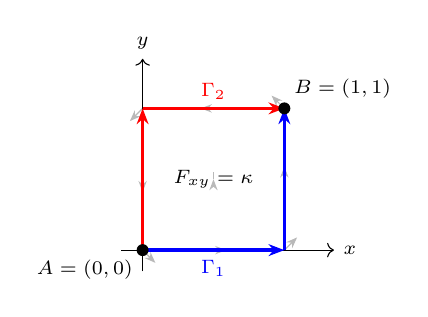
\begin{tikzpicture}[scale=1.8]
% field arrows (rotational)
\foreach \x in {0,0.5,1} {
  \foreach \y in {0,0.5,1} {
    \draw[gray!55,-{Stealth[length=1.4mm]}] (\x,\y) -- ++({-0.18*(\y-0.5)-0.0},{0.18*(\x-0.5)+0.0});
  }
}
% unit square axes
\draw[->] (-0.15,0) -- (1.35,0) node[right] {\scriptsize $x$};
\draw[->] (0,-0.15) -- (0,1.35) node[above] {\scriptsize $y$};
% route Gamma_1 : right then up (blue)
\draw[blue,very thick,-{Stealth[length=2mm]}] (0,0) -- (1,0);
\draw[blue,very thick,-{Stealth[length=2mm]}] (1,0) -- (1,1);
\node[blue] at (0.5,-0.13) {\scriptsize $\Gamma_1$};
% route Gamma_2 : up then right (red)
\draw[red,very thick,-{Stealth[length=2mm]}] (0,0) -- (0,1);
\draw[red,very thick,-{Stealth[length=2mm]}] (0,1) -- (1,1);
\node[red] at (0.5,1.12) {\scriptsize $\Gamma_2$};
% kernels
\fill (0,0) circle (1.2pt); \node[below left] at (0,0) {\scriptsize $A=(0,0)$};
\fill (1,1) circle (1.2pt); \node[above right] at (1,1) {\scriptsize $B=(1,1)$};
\node at (0.5,0.5) {\scriptsize $F_{xy}=\kappa$};
\end{tikzpicture}
\caption{\textbf{A two-kernel example in which the line integral is demonstrably path-dependent}}
\label{fig:worked}
\vspace{0.4em}
\begin{minipage}{0.95\textwidth}
\justifying\small
Two kernels sit at $A=(0,0)$ and $B=(1,1)$ in a flat plane. The grey arrows show the rotational thermal-flux potential $A_x=-\tfrac{\kappa}{2}y$, $A_y=+\tfrac{\kappa}{2}x$ of Eq.~\eqref{eq:worked-A}, whose field strength is the constant $F_{xy}=\kappa$. The blue route $\Gamma_1$ (right, then up) gives $\mathcal{S}_{\Gamma_1}=+\kappa/2$; the red route $\Gamma_2$ (up, then right) gives $\mathcal{S}_{\Gamma_2}=-\kappa/2$. The two disagree by exactly $\kappa$, the flux of $F_{xy}$ through the enclosed unit square. When $\kappa=0$ the potential is a pure gradient and both routes agree, so path-dependence is controlled entirely by $F_{\mu\nu}$.
\end{minipage}
\end{figure*}

% ========================================
% Section 14: Preliminary verifications of the roadmap steps
% ========================================
\section{Preliminary verifications of the roadmap steps}
\label{app:checks}

The roadmap of Sec.~\ref{sec:outlook} lists checks that are, in principle, computable. Three of them can already be carried out at the level of the geometric machinery, and we record the results here. These confirm that the machinery is internally consistent and that it reproduces the expected curvature signatures on concrete metrics; what they do \emph{not} yet do is establish the same facts for the specific 0-Sphere thermal-geodesic action $\mathcal{S}$, which requires that action in closed form and is deferred to a dedicated paper. All three were verified symbolically.

\paragraph{Check 1: metric reconstruction and the eikonal identity.}
In flat two-dimensional space the world function is $\mathcal{S}=\tfrac12[(x_B-x_A)^2+(y_B-y_A)^2]$, and the reconstruction~\eqref{eq:metric-recon} returns
\begin{equation}
-\,\partial_{A\mu}\partial_{B\nu}\,\mathcal{S} \;=\; \delta_{\mu\nu},
\label{eq:check1-metric}
\end{equation}
the correct Euclidean metric, while the eikonal identity~\eqref{eq:eikonal} holds exactly, $|\partial_B\mathcal{S}|^2=(x_B-x_A)^2+(y_B-y_A)^2=2\mathcal{S}$. On a sphere of radius $a$, in geodesic polar coordinates where $\sigma=\tfrac12 r^2$, the radial eikonal also holds exactly, $(\partial_r\sigma)^2=r^2=2\sigma$. The reconstruction route is therefore self-consistent in both the flat and the curved case. This closes, at the level of the geometric machinery, a check that earlier work left open: the draft that first proposed the metric-recovery formula explicitly deferred the explicit evaluation of $\partial_{A\mu}\partial_{B\nu}\mathcal{S}_s$ that demonstrates the flat-space limit~\cite{hanamura51}, recording it as a pending task; the computation above supplies it for the world-function form of $\mathcal{S}$, leaving only the substitution of the specific thermal-geodesic action for a dedicated paper.

\paragraph{Check 2: the van Vleck--Morette determinant carries the Ricci tensor.}
On a sphere of radius $a$ the determinant has the closed form $\Delta=(r/a)/\sin(r/a)$, whose small-distance expansion is
\begin{equation}
\Delta \;=\; 1 \;+\; \frac{1}{6}\Big(\frac{r}{a}\Big)^2 \;+\; \frac{7}{360}\Big(\frac{r}{a}\Big)^4 \;+\; \cdots
\label{eq:check2-expand}
\end{equation}
Since the Ricci tensor on the sphere satisfies $R_{\mu\nu}u^\mu u^\nu=1/a^2$ for a unit tangent, the leading deviation is exactly
\begin{equation}
\Delta - 1 \;=\; \frac{1}{6}\,R_{\mu\nu}\,u^\mu u^\nu\,r^2 \;+\; \mathcal{O}(r^4),
\label{eq:check2-ricci}
\end{equation}
confirming the central claim of Sec.~\ref{sec:bundle}: the first departure of the geodesic bundle from uniformity is governed by the Ricci tensor.

\paragraph{Check 3: the gradient and rotational sectors of $A_\mu$.}
For the worked connection of Appendix~\ref{app:worked}, $A=(-\tfrac{\kappa}{2}y,\,\tfrac{\kappa}{2}x)$, the field strength is $F_{xy}=\kappa$ while the divergence vanishes, $\partial_\mu A^\mu=0$: this $A_\mu$ is purely rotational and carries no gradient (pure-gauge) part. Conversely, any pure gradient $A_\mu=\partial_\mu\chi$ gives $F_{\mu\nu}=0$ identically. Helmholtz decomposition thus splits $A_\mu$ into an integrable gradient piece, which aligns with the metric sector, and a rotational piece whose curvature $F_{\mu\nu}$ is the genuinely new, non-metric content; by Stokes' theorem its holonomy equals the enclosed flux, $\oint A=\iint F_{xy}\,dA=\kappa$, reproducing the path difference of Appendix~\ref{app:worked}. The consistency check of Sec.~\ref{sec:reconcile} is therefore sharpened: the two doors agree on the gradient sector, and the rotational sector $F_{\mu\nu}$ is precisely where any torsion-like, beyond-metric structure would reside.

% ========================================
% Section 15: A short dictionary: three languages for the same ideas
% ========================================
\section{A short dictionary: three languages for the same ideas}
\label{app:dictionary}

This paper deliberately speaks three languages at once: the standard vocabulary of general relativity, the vocabulary of the 0-Sphere model, and ordinary words. A reader fluent in one of them can use Table~\ref{tab:dictionary} to translate into the others. The table is meant to be read row by row; each row is a single idea wearing three different costumes. Nothing in it is a new claim---it is a reading aid, gathering in one place the correspondences that the main text introduces as it goes.

% ----------------------------------------
% Table 3
% ----------------------------------------
\begin{table*}[t!]
\centering
\caption{\textbf{A reader's dictionary across the three languages of this paper}}
\label{tab:dictionary}
\renewcommand{\arraystretch}{1.35}
\begin{tabular}{p{4.6cm}p{5.2cm}p{6.0cm}}
\toprule
\textbf{General relativity} & \textbf{0-Sphere model} & \textbf{In plain words} \\
\midrule
Zero-sphere $S^0=\{x,x'\}$ (two points)
& The two kernels $A$ and $B$
& The two radiating sources, the discrete substrate everything is built on \\
\addlinespace[0.2cm]
World function $\sigma(x,x')=\tfrac12 d^2$
& Two-point action $\mathcal{S}(A,B)=\int_\Gamma A_\mu dx^\mu$
& The single number summarizing the path between the two kernels \\
\addlinespace[0.2cm]
Geodesic
& Thermal geodesic
& The preferred path the heat-like process actually selects \\
\addlinespace[0.2cm]
Metric $g_{\mu\nu}=-\partial_\mu\partial_{\nu'}\sigma$
& Emergent metric $g_{\mu\nu}=\partial_{A}\partial_{B}\mathcal{S}$
& The local rule for distance, read off the two-point action by differentiating twice \\
\addlinespace[0.2cm]
Geodesic congruence
& Bundle of neighboring thermal-exchange paths
& A whole family of side-by-side paths, not just one \\
\addlinespace[0.2cm]
van Vleck--Morette determinant $\Delta$
& Focusing measure of the bundle
& How much the family bunches together or spreads apart, relative to flat space \\
\addlinespace[0.2cm]
Raychaudhuri equation
& Focusing law of the thermal bundle
& The equation saying curvature is what makes the family converge \\
\addlinespace[0.2cm]
Ricci term $R_{\mu\nu}u^\mu u^\nu$
& Curvature felt by the bundle
& The bending that pulls neighboring paths together on average \\
\addlinespace[0.2cm]
Connection $A_\mu$ (or $\Gamma$)
& Integrand of the line integral / thermal-flux potential
& The rule for keeping a transported state ``pointing the same way'' \\
\addlinespace[0.2cm]
Field strength $F_{\mu\nu}=\partial_\mu A_\nu-\partial_\nu A_\mu$
& Path-dependence of $\mathcal{S}$
& How much the two-point answer depends on which route you take \\
\addlinespace[0.2cm]
Holonomy / Wilson loop
& Leftover phase around a closed exchange loop
& The twist a compass picks up after going around and coming back \\
\addlinespace[0.2cm]
Riemann tensor $R^\rho{}_{\sigma\mu\nu}$
& Full curvature of the kernel network
& The complete description of how transport around a loop fails to close \\
\addlinespace[0.2cm]
Principal $U(1)$ fibre bundle over $S^1$
& Internal phase circle with a winding fibre at each point
& The space of ``how the internal phase can twist'' along the one path \\
\addlinespace[0.2cm]
Geodesic congruence (\emph{not used physically})
& Internal winding family / chirality $\chi=\mathrm{sign}(da/dt)$
& The genuine family: the sense and number of internal twists, not side-by-side paths \\
\addlinespace[0.2cm]
Sectional / Ricci curvature (gravitational part)
& $\pi$-periodic Thomas vortex $\Omega_T\propto\tfrac12\sin 2\theta$ (spin-2)
& The real internal swirl whose winding carries the gravitational content \\
\addlinespace[0.2cm]
Stress-energy source / graviton exchange
& Ejected photon-sphere fragment ($\hbar\omega$) and entropic synchronisation
& The actual quantum the vortex throws to a neighbour, making a force \\
\bottomrule
\end{tabular}
\vspace{0.2cm}
\begin{minipage}{0.95\textwidth}
\justifying\footnotesize
Each row is one idea in three languages. The upper block (down to the Riemann tensor) belongs to the geometric reading of the two doors: distance function $\to$ metric $\to$ curvature, and connection $\to$ field strength $\to$ holonomy $\to$ Riemann. The lower block records the physical correction of Sec.~\ref{sec:bundle}: because the thermal geodesic is unique, the family that reveals curvature is not a spatial geodesic congruence but the internal winding---the chirality fibre and its Thomas-precession vortex---whose $\pi$-periodic, spin-2 component carries the gravitational content. The geodesic congruence and the van Vleck--Morette / Raychaudhuri calculus remain valid as mathematics once a metric field exists, but are not the physical mechanism here.
\end{minipage}
\end{table*}

% ========================================
% Acknowledgments
% ========================================
\begin{acknowledgments}
The author acknowledges the use of a large language model in a supportive role for textual organization, mathematical consultation, and structural analysis of the relationships among earlier papers in the series. All physical interpretations, theoretical claims, and conclusions are the sole responsibility of the author.
\end{acknowledgments}

\clearpage

% ========================================
% Bibliography
% ========================================
\begin{thebibliography}{99}

\bibitem{hanamura24}
S.~Hanamura,
``Thermal Geodesics in the 0-Sphere Model: Extending General Relativity Through Internal Thermodynamic Structure,''
Zenodo (2025).
\href{https://doi.org/10.5281/zenodo.17765349}{https://doi.org/10.5281/zenodo.17765349}

\bibitem{hanamura29}
S.~Hanamura,
``Geometric Structure of Spinorial Phase Accumulation along Thermal Geodesics,''
Zenodo (2025).
\href{https://doi.org/10.5281/zenodo.18067760}{https://doi.org/10.5281/zenodo.18067760}

\bibitem{hanamura30}
S.~Hanamura,
``From Curvature to Connection: Revisiting the Geometric Origin of Conservation Laws,''
Zenodo (2026).
\href{https://doi.org/10.5281/zenodo.18819682}{https://doi.org/10.5281/zenodo.18819682}

\bibitem{hanamura31}
S.~Hanamura,
``Line Integrals as Fundamental Observables in Physics: A Unified Principle Behind the Aharonov-Bohm Effect, Berry Phase, and Wilson Loops,''
Zenodo (2026).
\href{https://doi.org/10.5281/zenodo.18203433}{https://doi.org/10.5281/zenodo.18203433}

\bibitem{hanamura40}
S.~Hanamura,
``On the Derivative-Order Mismatch Between Gauge Theory and Gravity: A Supplement on Connection, Curvature, and Line-Integral Observables,''
Zenodo (2026).
\href{https://doi.org/10.5281/zenodo.18736670}{https://doi.org/10.5281/zenodo.18736670}

\bibitem{hanamura41}
S.~Hanamura,
``A Note on Derivative Hierarchy in Gauge Theory and Gravity: A Historical Supplement on Connection, Curvature, and Line-Integral Observables,''
Zenodo (2026).
\href{https://doi.org/10.5281/zenodo.18809117}{https://doi.org/10.5281/zenodo.18809117}

\bibitem{hanamura55}
S.~Hanamura,
``Four Functions of the Open Wilson Line in the 0-Sphere Model: Phase-History Carrier, Gauge Localization, Holonomy Composition, and Boundary Data Generating Both Maxwell and Metric Sectors,''
Zenodo (2026).
\href{https://doi.org/10.5281/zenodo.19800797}{https://doi.org/10.5281/zenodo.19800797}

\bibitem{hanamura51}
S.~Hanamura,
``Helical Trajectory, Fixed-Endpoint Line Integrals, and the Emergence of the Spacetime Metric in the 0-Sphere Model,''
Zenodo (2026), revised version.
\href{https://doi.org/10.5281/zenodo.20388056}{https://doi.org/10.5281/zenodo.20388056}

\bibitem{MTW1973} C.~W.~Misner, K.~S.~Thorne, and J.~A.~Wheeler, \textit{Gravitation} (W.~H.~Freeman, San Francisco, 1973).

\bibitem{Synge1960} J.~L.~Synge, \textit{Relativity: The General Theory} (North-Holland, Amsterdam, 1960).

\bibitem{hanamura50}
S.~Hanamura,
``Rotation from Scalar Oscillation: Emergence of Photon-Sphere Angular Momentum from Phase-Staggered Kernel Dynamics in the 0-Sphere Model,''
Zenodo (2026).
\href{https://doi.org/10.5281/zenodo.19482145}{https://doi.org/10.5281/zenodo.19482145}

\bibitem{hanamura48}
S.~Hanamura,
``Geometric Origin of $g = 2$ in the 0-Sphere Model: U(1) Fiber Bundle and Dual-Frame Phase Decomposition,''
Zenodo (2026).
\href{https://doi.org/10.5281/zenodo.19227518}{https://doi.org/10.5281/zenodo.19227518}

\bibitem{hanamura49}
S.~Hanamura,
``Photon-Sphere Fragmentation as a Gravitational Mediator: Radiation-Gradient Ejection in the $\pi$-Cycle of the 0-Sphere Model,''
Zenodo (2026).
\href{https://doi.org/10.5281/zenodo.19393391}{https://doi.org/10.5281/zenodo.19393391}

\bibitem{hanamura34}
S.~Hanamura,
``Geometrical Confinement of Energy in the 0-Sphere Model: A Topological Mechanism Underlying Rest Mass, Zitterbewegung, and Gravitational-Like Phenomena,''
Zenodo (2026).
\href{https://doi.org/10.5281/zenodo.18437010}{https://doi.org/10.5281/zenodo.18437010}

\bibitem{hanamura22}
S.~Hanamura,
``Gravitational Redshift of Internal Quantum Clocks: A Zitterbewegung-Based Model,''
Zenodo (2025).
\href{https://doi.org/10.5281/zenodo.17765318}{https://doi.org/10.5281/zenodo.17765318}

\bibitem{Kothawala2023} D.~Kothawala, \textit{Minimal length and small scale structure of spacetime}, Phys.\ Rev.\ D \textbf{88}, 104029 (2013); D.~Kothawala and T.~Padmanabhan, \textit{Grin of the Cheshire cat: Entropy density of spacetime as a relic from quantum gravity}, Phys.\ Rev.\ D \textbf{90}, 124060 (2014).

\bibitem{hanamura19}
S.~Hanamura,
``Spin as a Real Vector from Internal Photon-Sphere Motion: Geometric Origin of U(1) Gauge and SU(2) Periodicity,''
Zenodo (2025).
\href{https://doi.org/10.5281/zenodo.17765238}{https://doi.org/10.5281/zenodo.17765238}

\bibitem{WuYang1975} T.~T.~Wu and C.~N.~Yang, \textit{Concept of nonintegrable phase factors and global formulation of gauge fields}, Phys.\ Rev.\ D \textbf{12}, 3845 (1975).

\bibitem{AharonovBohm1959} Y.~Aharonov and D.~Bohm, \textit{Significance of electromagnetic potentials in the quantum theory}, Phys.\ Rev.\ \textbf{115}, 485 (1959).

\bibitem{Berry1984} M.~V.~Berry, \textit{Quantal phase factors accompanying adiabatic changes}, Proc.\ R.\ Soc.\ Lond.\ A \textbf{392}, 45 (1984).

\bibitem{hanamura54}
S.~Hanamura,
``Maxwell Electrodynamics as a Derived Low-Energy Limit of the 0-Sphere Line-Integral Ontology,''
Zenodo (2026).
\href{https://doi.org/10.5281/zenodo.19701297}{https://doi.org/10.5281/zenodo.19701297}

\bibitem{hanamura60}
S.~Hanamura,
``The Berry--Synge--Bonnet--Myers Triangle: Structural Conditions for the Unification of Gauge and Gravitational Sectors in the 0-Sphere Model,''
Zenodo (2026).
\href{https://doi.org/10.5281/zenodo.19932922}{https://doi.org/10.5281/zenodo.19932922}

\bibitem{hanamura53}
S.~Hanamura,
``From Gravitational Mediation to Directional Force Classification: A Conceptual and Mathematical Supplement to Papers \#49, \#50, \#51, and \#52 of the 0-Sphere Model Series,''
Zenodo (2026).
\href{https://doi.org/10.5281/zenodo.19616971}{https://doi.org/10.5281/zenodo.19616971}

\bibitem{hanamura46}
S.~Hanamura,
``Geometric Origin of the One-Half Factor: Thermal Potential Energy Floor and Zero-Point Energy in the 0-Sphere Model: A Conceptual Clarification,''
Zenodo (2026).
\href{https://doi.org/10.5281/zenodo.19010945}{https://doi.org/10.5281/zenodo.19010945}

\bibitem{DeWitt1960} B.~S.~DeWitt and R.~W.~Brehme, \textit{Radiation damping in a gravitational field}, Ann.\ Phys.\ (N.Y.) \textbf{9}, 220 (1960).

\bibitem{Poisson2011} E.~Poisson, A.~Pound, and I.~Vega, \textit{The motion of point particles in curved spacetime}, Living Rev.\ Relativity \textbf{14}, 7 (2011).

\bibitem{VanVleck1928} J.~H.~Van Vleck, \textit{The correspondence principle in the statistical interpretation of quantum mechanics}, Proc.\ Natl.\ Acad.\ Sci.\ USA \textbf{14}, 178 (1928).

\bibitem{Morette1951} C.~Morette, \textit{On the definition and approximation of Feynman's path integrals}, Phys.\ Rev.\ \textbf{81}, 848 (1951).

\bibitem{Visser1993} M.~Visser, \textit{van Vleck determinants: Geodesic focusing and defocusing in Lorentzian spacetimes}, Phys.\ Rev.\ D \textbf{47}, 2395 (1993).

\bibitem{Raychaudhuri1955} A.~K.~Raychaudhuri, \textit{Relativistic cosmology. I}, Phys.\ Rev.\ \textbf{98}, 1123 (1955).

\bibitem{Nakahara2003} M.~Nakahara, \textit{Geometry, Topology and Physics}, 2nd ed.\ (Institute of Physics Publishing, Bristol, 2003).

\end{thebibliography}

% ========================================
% End of Document
% ========================================
\end{document}
